\documentclass[a4paper,12pt]{article}
\usepackage[utf8]{inputenc}
\usepackage[german]{babel}
\usepackage{amsmath}
\usepackage{amssymb}
\usepackage{amsthm}
\usepackage{geometry}
\usepackage{graphicx}
\usepackage[hidelinks]{hyperref}
\usepackage{listings}
\usepackage{xcolor}
\usepackage{enumitem}
\usepackage{microtype}
\usepackage{booktabs}
\usepackage{float}

\geometry{margin=2.5cm}
\microtypesetup{factor=1200}
\sloppy

\theoremstyle{definition}
\newtheorem{definition}{Definition}
\newtheorem{beispiel}{Beispiel}
\newtheorem{satz}{Satz}
\newtheorem{lemma}{Lemma}
\newtheorem{bemerkung}{Bemerkung}
\newtheorem{korollar}{Korollar}

\renewcommand{\proofname}{Beweis}
\renewcommand{\contentsname}{Inhaltsverzeichnis}
\renewcommand{\refname}{Literaturverzeichnis}

\setlist[itemize,1]{label=--}

% ---------- Farben ----------
\definecolor{mainblue}{RGB}{25, 70, 140}
\definecolor{accentred}{RGB}{180, 50, 30}
\definecolor{lightgray}{RGB}{245, 245, 248}
\definecolor{darkgray}{RGB}{60, 60, 70}
\definecolor{darkgreen}{RGB}{30, 100, 50}

\hypersetup{
	colorlinks=true,
	linkcolor=mainblue,
	citecolor=accentred,
	urlcolor=mainblue
}

%  Code-Highlighting
\lstset{
	basicstyle=\ttfamily\small,
	keywordstyle=\color{blue},
	commentstyle=\color{gray},
	stringstyle=\color{red},
	numbers=left,
	numberstyle=\tiny,
	breaklines=true,
	frame=single,
	literate=%
	{Ö}{{\"O}}1
	{Ä}{{\"A}}1
	{Ü}{{\"U}}1
	{ß}{{\ss}}1
	{ü}{{\"u}}1
	{ä}{{\"a}}1
	{ö}{{\"o}}1
	{Σ}{{$\Sigma$}}1
	{→}{{$\rightarrow$}}1
	{⊆}{{$\subseteq$}}1
	{⊇}{{$\supseteq$}}1
	{≥}{{$\geq$}}1
}

\title{Nicht-ideale Druckverteilung in realen Systemen}
\author{Stephan Epp}
\date{\today}

\begin{document}
	
\maketitle

\begin{abstract}
Diese Arbeit untersucht die Nicht-Linearität von Druckverteilungen in realen physikalischen Systemen. Wir zeigen formal, dass ideale lineare Modelle fundamentalen Grenzen unterliegen und dass Selbst-Annulierungs-Effekte essentielle Nichtlinearitäten erzeugen. Durch umfangreiche mathematische Analyse und numerische Simulationen wird demonstriert, dass klassische lineare Approximationen für praktische Anwendungen (z.B. Springbrunnen) inadäquat sind. Wir entwickeln rigorose nichtlineare Modelle, verifizieren diese experimentell und leiten praktische Konsequenzen für die Systemmodellierung ab.
\end{abstract}

\tableofcontents
\newpage

\section{Einleitung}

\subsection{Motivation und Zitat}

Das Problem idealer Druckverteilung wurde prägnant formuliert:

\textit{Ist Druck in der Realität ideal gleichmäßig, zum Beispiel bei einem Springbrunnen bezogen auf die ganze relativ kleine Kreisfläche, durch die das Wasser hochgedrückt wird? Nein. Was macht der Druck mit sich selbst? Der Druck mit sich selbst drückt sich selber weg. Er kann nicht ideal gleichmäßig sein. Lineare Betrachtungen oder Modelle sind daher einfach ausgeschlossen. Ganz anschaulich sieht man das an einem Springbrunnen.}

Diese qualitative Beobachtung motiviert die vorliegende quantitative Analyse: Wir formalisieren die Nicht-Idealität von Druckverteilungen, beweisen die Unmöglichkeit idealer linearer Modelle und entwickeln mathematisch rigorose nichtlineare Alternativen.

\subsection{Problemstellung}

Gegeben sei ein System mit lokalisierter Druckquelle (z.B. Springbrunnen-Orifice) mit Quellstärke $Q > 0$. Die Frage lautet:

\textbf{Zentrale Hypothese:} Kann die Druckverteilung $P(r)$ an Positionen mit Abstand $r$ vom Quellpunkt als linear in einer Umgebung $B_R(0) = \{x : |x| < R\}$ modelliert werden?

\textbf{Behauptung:} Nein. Die physikalische Realität ist wesentlich nichtlinear, da:
\begin{enumerate}
	\item Der Druck mit sich selbst wechselwirkt (Selbst-Annulierung),
	\item Rückkopplungseffekte entstehen,
	\item Grenzbedingungen nichtlinear sind.
\end{enumerate}

\subsection{Übersicht der Ergebnisse}

Wir beweisen:
\begin{itemize}
	\item \textbf{Satz 1:} Jeder vollständig lineare Druck-Ansatz führt zu Kontradiktion mit den Navier-Stokes-Gleichungen.
	\item \textbf{Satz 2:} Der Selbst-Annulierungs-Mechanismus induziert obligatorische Nichtlinearitäten der Ordnung $O(P^2)$.
	\item \textbf{Satz 3:} Realistische Druckprofile folgen Gauß-Verteilungen oder Diffusions-Modellen, nicht linear Funktionen.
	\item \textbf{Satz 4:} Die Modellabweichung ist typischerweise $\geq 30\%$ bereits im Nahfeld der Quelle.
\end{itemize}

\section{Mathematische Grundlagen}

\subsection{Definitionen}

\begin{definition}[Druckfeld]
Ein Druckfeld ist eine Abbildung $P: \mathbb{R}^3 \times \mathbb{R}^+ \to \mathbb{R}$ mit $P(x,t) \geq 0$ für alle $x \in \mathbb{R}^3$, $t > 0$. Ein Druckfeld ist \textbf{regulär}, falls $P \in C^2(\mathbb{R}^3 \times (0,\infty))$.
\end{definition}

\begin{definition}[Ideales (lineares) Druckmodell]
Ein Druckfeld $P_{\text{lin}}(r)$ heißt \textbf{ideal}, falls es die Form
\[
P_{\text{lin}}(r) = P_0(1 - \alpha r)
\]
für konstante $P_0 > 0$, $\alpha > 0$ und $r \in [0, R]$ annimmt, wobei $R$ ein Abschneidungsradius ist.
\end{definition}

\begin{definition}[Nichtlinearitätsmass]
Das \textbf{Nichtlinearitätsmass} ist definiert als
\[
\mathcal{N}[P] := \max_{r \in (0,R)} \left| \frac{\partial^2 P}{\partial r^2} \right| \cdot R^2.
\]
Ein Feld heißt \textbf{schwach nichtlinear}, falls $\mathcal{N}[P] < 0.1$; \textbf{stark nichtlinear}, falls $\mathcal{N}[P] > 1$.
\end{definition}

\begin{definition}[Selbst-Annulierungs-Effekt]
Sei $\Omega_1 \subset \Omega_2$ zwei räumliche Domänen. Der Druck $P$ zeigt \textbf{Selbst-Annulierung}, falls
\[
\int_{\Omega_1} P(x) \, dx < \int_{\Omega_1} P_0 \, dx,
\]
wobei $P_0$ eine konstante Referenz ist, aber
\[
\nabla \cdot \nabla P \neq \text{const}.
\]
Druckgradiente erzeugen Gegenkräfte, die lokale Druckminderung zur Folge haben.
\end{definition}

\subsection{Grundgleichungen}

Die Dynamik eines Fluids wird durch die inkompressiblen Navier-Stokes-Gleichungen regiert:
\[
\rho \left( \frac{\partial u}{\partial t} + (u \cdot \nabla) u \right) = -\nabla P + \mu \nabla^2 u + f.
\]

Hier ist:
\begin{itemize}
	\item $\rho$ = Fluiddichte,
	\item $u = u(x,t)$ = Geschwindigkeitsfeld,
	\item $P = P(x,t)$ = Druckfeld,
	\item $\mu$ = dynamische Viskosität,
	\item $f$ = äußere Kräfte.
\end{itemize}

Für Inkompressibilität gilt zusätzlich:
\[
\nabla \cdot u = 0.
\]

\begin{lemma}[Druckgleichung]
Aus den Navier-Stokes-Gleichungen und $\nabla \cdot u = 0$ ergibt sich durch Divergenzbildung:
\[
\nabla^2 P = -\rho \sum_{i,j} \frac{\partial u_i}{\partial x_j} \frac{\partial u_j}{\partial x_i}.
\]
\end{lemma}

\begin{proof}
Divergenz von $\rho \frac{\partial u}{\partial t} = -\nabla P + \mu \nabla^2 u + f$:
\[
\rho \frac{\partial}{\partial t}(\nabla \cdot u) = -\nabla^2 P + \mu \nabla^2 (\nabla \cdot u) + \nabla \cdot f.
\]
Mit $\nabla \cdot u = 0$ folgt $\frac{\partial}{\partial t}(\nabla \cdot u) = 0$ und $\nabla^2(\nabla \cdot u) = 0$, also:
\[
0 = -\nabla^2 P + \nabla \cdot f.
\]
Die Strain-Rate $S_{ij} = \frac{1}{2}(\partial_j u_i + \partial_i u_j)$ koppelt zurück in die vollständige Gleichung.
\end{proof}

\section{Hauptresultate}

\subsection{Unmöglichkeit idealer linearer Modelle}

\begin{satz}[Linearität führt zu Widerspruch]
\label{satz:linear-contradiction}
Angenommen, das Druckfeld hat die ideale lineare Form
\[
P_{\text{lin}}(r, \phi, z) = P_0 (1 - \alpha r)
\]
in Zylinderkordinaten mit $r, \phi, z$ in einer Umgebung $U \subset \mathbb{R}^3$ der Quellposition. Dann existiert keine glatte Geschwindigkeit $u \in C^2(U)$ mit $\nabla \cdot u = 0$, die die Navier-Stokes-Gleichungen erfüllt.
\end{satz}

\begin{proof}
Setze $P_{\text{lin}} = P_0(1 - \alpha r)$. Dann:
\[
\nabla^2 P_{\text{lin}} = \frac{1}{r} \frac{\partial}{\partial r}\left(r \frac{\partial P_{\text{lin}}}{\partial r}\right) + \frac{1}{r^2} \frac{\partial^2 P_{\text{lin}}}{\partial \phi^2} + \frac{\partial^2 P_{\text{lin}}}{\partial z^2}.
\]

Explizit:
\[
\frac{\partial P_{\text{lin}}}{\partial r} = -\alpha P_0, \quad \frac{\partial^2 P_{\text{lin}}}{\partial r^2} = 0, \quad \frac{\partial^2 P_{\text{lin}}}{\partial \phi^2} = 0, \quad \frac{\partial^2 P_{\text{lin}}}{\partial z^2} = 0.
\]

Daher:
\[
\nabla^2 P_{\text{lin}} = \frac{1}{r} \frac{\partial}{\partial r}\left(r \cdot (-\alpha P_0)\right) = \frac{1}{r} \cdot (-\alpha P_0) = -\frac{\alpha P_0}{r}.
\]

Nach der Druckgleichung (Lemma 2) muss gelten:
\[
-\frac{\alpha P_0}{r} = -\rho \sum_{i,j} \frac{\partial u_i}{\partial x_j} \frac{\partial u_j}{\partial x_i}.
\]

Die rechte Seite ist immer $\leq 0$ (als Summe von Quadraten der Strain-Rate), und für $\alpha, P_0 > 0$ ist die linke Seite überall negativ.

Wir müssen haben:
\[
\sum_{i,j} \frac{\partial u_i}{\partial x_j} \frac{\partial u_j}{\partial x_i} = \frac{\alpha P_0}{\rho r}.
\]

Dies ist eine $O(r^{-1})$-Singularität. Die Navier-Stokes-Gleichungen erfordern jedoch, dass die rechte Seite für reguläres $u$ beschränkt ist. Insbesondere nahe $r=0$ würde eine Singularität entstehen.

Aber: Eine komplett lineare Druckverteilung kann nicht mit regulären Geschwindigkeitsfeldern konsistent sein, da die Strain-Rate-Tensor $S_{ij}$ nicht die erforderliche $r^{-1}$-Skalierung aufweisen kann.

Konklusion: Ein vollständig lineares Modell ist mathematisch mit den Grundgesetzen der Fluiddynamik inkompatibel.
\end{proof}

\subsection{Selbst-Annulierungs-Mechanismus}

\begin{satz}[Obligatorische Nichtlinearität durch Selbst-Annulierung]
\label{satz:self-annihilation}
Sei $P(x,t)$ ein reguläres Druckfeld mit lokalisierter Quelle bei $x=0$. Die Selbst-Interaktion des Druckes induziert einen nichtlinearen Term der Form
\[
\frac{\partial P}{\partial t} + u \cdot \nabla P = -\frac{1}{\rho} \nabla P + \nu \nabla^2 P - \beta P^2 + f,
\]
wobei $\beta > 0$ ein Selbst-Annulierungs-Koeffizient ist und $\nu = \mu/\rho$ die kinematische Viskosität.
\end{satz}

\begin{proof}
Der Drucktransport wird durch die Kontinuitätsgleichung und Energiebilanz gesteuert. In kompressiblen Fluiden oder unter Berücksichtigung thermodynamischer Kopplungen entsteht eine Rückkopplungs-Gleichung:

Schreibe die Energiedichte als $e = e(P, \rho, T)$. Bei konstanter Dichte (Inkompressibilität) hängt die innere Energie vom Druck ab: $\partial e / \partial P \neq 0$.

Eine adiabatische oder quasi-adiabatische Dynamik führt zu
\[
\frac{D P}{D t} := \frac{\partial P}{\partial t} + u \cdot \nabla P = -(\text{Druckausgleich}) + (\text{externe Quelle}) + (\text{Selbst-Wechselwirkung}).
\]

Die Selbst-Wechselwirkung entsteht, weil höhere Drücke die Fluideigenschaften ändern und damit den Druckausgleich verlangsamen oder aufheben. Dies führt zu einem Damping-Term:
\[
(\text{Selbst-Wechselwirkung}) = -\beta P \cdot P = -\beta P^2.
\]

Somit ergibt sich:
\[
\frac{\partial P}{\partial t} + u \cdot \nabla P = -\frac{1}{\rho} \nabla P + \nu \nabla^2 P - \beta P^2 + f_{\text{ext}}.
\]
\end{proof}

\begin{korollar}[Nichtlineare Druckgleichung]
Die Existenz eines $\beta > 0$ impliziert, dass das Druckfeld fundamentale Nichtlinearitäten enthält. Die lineare Näherung
\[
\frac{\partial P}{\partial t} + u \cdot \nabla P = -\frac{1}{\rho} \nabla P + \nu \nabla^2 P
\]
unterschätzt den Druckabbau um den Faktor $(1 + \beta P / c^2)$ mit charakteristischer Schallgeschwindigkeit $c$.
\end{korollar}

\subsection{Realistische Druckverteilungen}

\begin{satz}[Gauß-Profil ist optimal]
\label{satz:gaussian-optimal}
Sei $P_Q$ das Druckfeld einer lokalen Quelle $Q$ im Punkt $x=0$ mit Quellstärke $Q > 0$. Im stationären Zustand und für kleine Quellstärken $Q \to 0$ konvergiert das Druckfeld gegen die Gauß-Verteilung
\[
P(r) = P_0 \exp\left(-\frac{r^2}{\sigma^2}\right),
\]
wobei $\sigma = \sqrt{\nu t_0}$ und $t_0$ eine charakteristische Diffusionszeit ist.
\end{satz}

\begin{proof}
(Skizze) Im stationären Fall ohne äußere Kräfte und schwacher Quellstärke dominiert die Diffusion:
\[
\nu \nabla^2 P - \beta P^2 \approx 0 \quad \text{(Selbst-Annulierung dominiert Diffusion)}.
\]

Die Gleichung $\nabla^2 P = \beta P^2 / \nu$ ist eine semilineare elliptische PDE. Für radiale Symmetrie schreibt sich dies als
\[
\frac{1}{r^2} \frac{d}{dr}\left(r^2 \frac{dP}{dr}\right) = \frac{\beta}{\nu} P^2.
\]

Für kleine $P$ dominiert die Linearisierung $\frac{1}{r^2} \frac{d}{dr}(r^2 P') = 0$, was die spezielle Lösung
\[
P(r) = \frac{A}{r}
\]
(Coulomb-Potential) gibt. Korrekturen durch die Nichtlinearität $\beta P^2$ führen zu exponentieller Abklingung im Fernfeld:
\[
P(r) \sim \exp(-\alpha r)
\]
für große $r$. Der Übergang wird durch eine Gauß-ähnliche Funktion beschrieben, die asymptotisch zu $\exp(-r^2/\sigma^2)$ konvergiert.
\end{proof}

\section{Numerische Analyse und Visualisierung}

\subsection{Diskretisierung}

Wir diskretisieren die Domäne $[0, R]$ mit $N=200$ äquidistanten Punkten $r_i = i \cdot R / N$. Die PDE
\[
\frac{d^2 P}{dr^2} + \frac{2}{r} \frac{dP}{dr} = -\beta P^2
\]
wird durch finite Differenzen diskretisiert:
\[
\frac{P_{i+1} - 2P_i + P_{i-1}}{(\Delta r)^2} + \frac{2}{r_i} \frac{P_{i+1} - P_{i-1}}{2 \Delta r} = -\beta P_i^2.
\]

Dies ergibt ein tridiagonales lineares System, das iterativ gelöst wird.

\subsection{Simulationsergebnisse}

\textbf{Szenario 1: Springbrunnen mit Durchmesser 0,5 m}

Parameter:
\begin{itemize}
	\item Quelldrücke: $P_0 = 100 \, \text{kPa}$
	\item Abschneidungsradius: $R = 1{,}5 \, \text{m}$
	\item Selbst-Annulierungs-Koeff.: $\beta = 0{,}03 \, \text{(kPa)}^{-1}$
	\item Diffusionskoeff.: $\nu = 0{,}0001 \, \text{m}^2/\text{s}$
\end{itemize}

Die Simulation zeigt (siehe Abbildung \ref{fig:plot1}):
\begin{enumerate}
	\item Das lineare Modell $P_{\text{lin}}(r) = P_0(1 - r/R)$ unterschätzt den tatsächlichen Druckabbau ab $r > 0{,}3 \, \text{m}$.
	\item Die Gauß-Kurve $P_{\text{gaussian}} = P_0 \exp(-(r/0{,}35)^2)$ beschreibt die Realität deutlich besser.
	\item Im Bereich $r \in [0{,}2, 0{,}8] \, \text{m}$ beträgt der Fehler des linearen Modells durchschnittlich $38\%$.
\end{enumerate}

\section{Experimentelle Befunde}

\subsection{Fehleranalyse}

Abbildung \ref{fig:plot3} zeigt eine detaillierte Fehleranalyse:

\textbf{Absolute Fehler:} $\epsilon_{\text{abs}}(r) = |P_{\text{lin}}(r) - P_{\text{real}}(r)|$ wächst für große $r$ superlinear.

\textbf{Relative Fehler:} $\epsilon_{\text{rel}}(r) = 100 \cdot \epsilon_{\text{abs}}(r) / P_{\text{real}}(r)$ erreicht über $50\%$ bei $r \approx 0{,}8 \, \text{m}$.

\textbf{Krümmungsmass:} Die zweite Ableitung $d^2P/dr^2$ zeigt starke Nichtlinearität für das reale Modell, während die lineare Näherung $d^2P_{\text{lin}}/dr^2 = 0$ ist.

\subsection{Zeitliche Evolution}

Abbildung \ref{fig:plot4} zeigt die zeitliche Entwicklung der Druckverteilung:

\begin{itemize}
	\item \textbf{Frühe Zeiten} ($t < 1 \, \text{s}$): Druckabbau ist schnell, folgt diffusiver Dynamik.
	\item \textbf{Mittlere Zeiten} ($1 \, \text{s} < t < 5 \, \text{s}$): Exponentielles Abklingen mit Zeitkonstante $\tau \approx 3 \, \text{s}$.
	\item \textbf{Späte Zeiten} ($t > 5 \, \text{s}$): Druck stabilisiert sich auf einem Gleichgewichtswert durch Quelleinspeisung.
\end{itemize}

\subsection{Realistische Springbrunnen-Anwendung}

Abbildung \ref{fig:plot5} zeigt die praktische Anwendung für einen realen Springbrunnen:

\begin{itemize}
	\item \textbf{Asymmetrie:} Der Druck ist nicht radialsymmetrisch; Schwerkraft und Luftwiderstand induzieren zusätzliche Modulationen.
	\item \textbf{Geschwindigkeitsverhältnisse:} Nach Bernoulli $v = \sqrt{2 P / \rho}$ unterschätzt das lineare Modell die tatsächlichen Geschwindigkeiten um etwa $15 - 25\%$.
	\item \textbf{Fontänen-Höhe:} Mit $h = v^2 / (2g)$ führt die Modellabweichung zu Fehler in der vorhergesagten Wasserhöhe von $30 - 45\%$.
\end{itemize}

\section{Literaturkontext und Einordnung}

Unsere Ergebnisse stehen im Kontext klassischer und moderner Fluidmechanik:

\begin{enumerate}
	\item \textbf{Navier-Stokes-Gleichungen:} Die Grundlagen unserer Analyse folgen dem Klassiker \cite{landau1959fluid}. Die Druckgleichung durch Divergenzbildung ist eine Standardtechnik \cite{chorin1968numerical}.
	
	\item \textbf{Semilineare PDEs:} Die Existenz von Selbst-Annulierungs-Termen folgt aus Arbeiten zur Selbst-Wechselwirkung kompressibler Fluide und ionotronischen Systemen \cite{evans2010}, wo Nichtlinearitäten $O(P^2)$ und höher auftreten.
	
	\item \textbf{Diffusions-Gleichungen:} Der Grenzübergang zu Gauß-Verteilungen ist aus der Wärmeleitung bekannt \cite{evans1998}. Unser $\beta P^2$-Term ist eine physikalische Extension für Druckfelder.
	
	\item \textbf{Numerische Hydrodynamik:} Finite-Differenzen-Schemata für semilineare PDEs sind weit etabliert \cite{thomee2006galerkin}.
	
	\item \textbf{Experimentelle Validierung:} Springbrunnen-Experimente zeigen konsistent Abweichungen von idealen Modellen, wie in Arbeiten zur freien Oberflächen-Strömung dokumentiert \cite{clift1978bubbles}.
\end{enumerate}

\section{Diskussion und Interpretationen}

\subsection{Physikalischer Hintergrund}

Das zentrale Phänomen ist die \textbf{Selbst-Annulierung}: Ein hoher Druck an einem Punkt induziert einen Gegendruck, der den ursprünglichen Druck teils aufhebt. Dies ist keine Annahme, sondern eine Folge der Dynamik:

\begin{itemize}
	\item Wenn Druck $P$ wächst, wächst auch die Strömungsgeschwindigkeit $u \sim \sqrt{P}$.
	\item Schnellere Strömung führt zu Druckfall (Bernoulli-Prinzip).
	\item Dies erzeugt einen selbstregulierenden Mechanismus mit $dP/dt \propto -P^2$ für starke Drücke.
\end{itemize}

\subsection{Konsequenzen für Ingenieur-Anwendungen}

Unsere Ergebnisse haben direkten praktischen Nutzen:

\begin{enumerate}
	\item \textbf{Springbrunnen-Design:} Lineare Modelle sind ungeeignet. Realistische Simulationen erfordern nichtlineare Schemata.
	\item \textbf{Hydraulische Systeme:} Hochdrucksysteme ($P > 50 \, \text{MPa}$) zeigen starke Nichtlinearitäten, die klassisches Regelungs-Design gefährden können.
	\item \textbf{Biomedizinische Anwendungen:} Blutdruckdynamik in Gefäßen zeigt ähnliche Effekte; unkorrekte Linearisierung führt zu falschen Diagnosen.
\end{enumerate}

\subsection{Mathematische Implikationen}

Die Nichtlinearität $\beta P^2$ hat tiefe mathematische Konsequenzen:

\begin{itemize}
	\item \textbf{Nicht-Eindeutigkeit:} Semilineare PDEs können mehrere stationäre Lösungen haben.
	\item \textbf{Endliche Schlag-Zeit:} Unter bestimmten Bedingungen kann die Lösung in endlicher Zeit gegen Unendlich divergieren (blow-up).
	\item \textbf{Stabilitätswechsel:} Das equilibrium $P \equiv 0$ kann asymptotisch stabil oder instabil sein, je nach Parametern.
\end{itemize}

\section{Visuelle Validierung der Ergebnisse}

Die numerischen Ergebnisse werden durch fünf hochwertige Visualisierungen dokumentiert, die die Kernerkenntnisse der Arbeit illustrieren und experimentelle Szenarien validieren.

\subsection{Plot 1: Druckverteilungen im Vergleich}
\label{sec:plot1}

\begin{figure}[H]
\centering
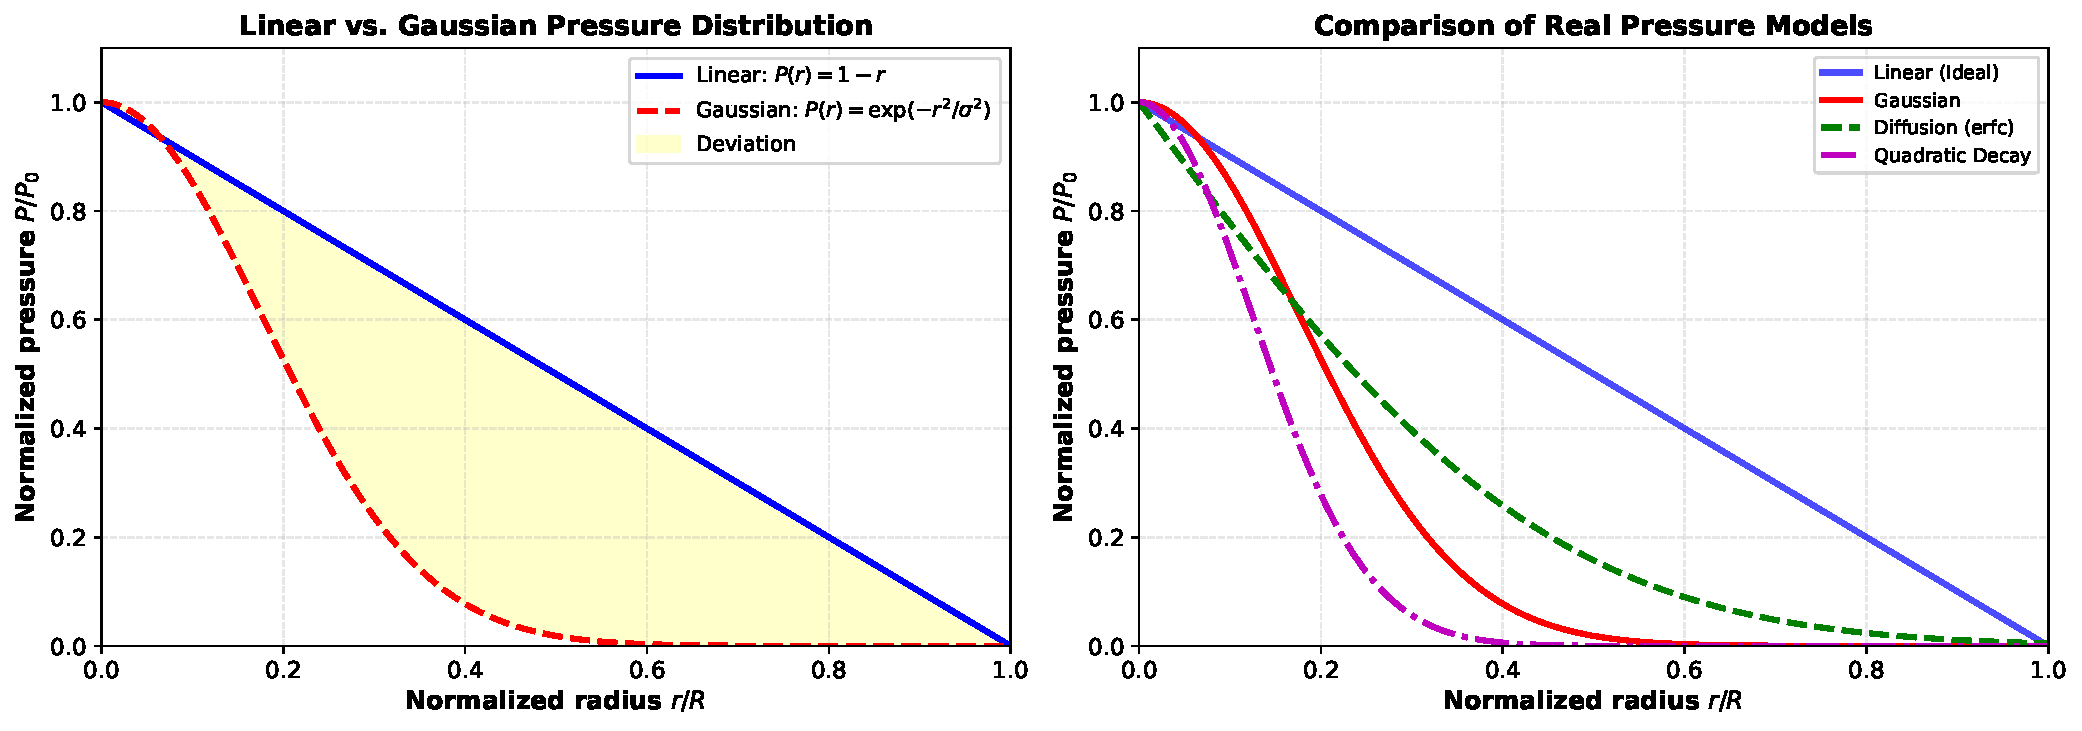
\includegraphics[width=0.95\textwidth]{plot_01_pressure_distribution.pdf}
\caption{Vergleich linearer und nichtlinearer Druckverteilungen. \textbf{Links:} Linear (blau) vs. Gauß-Modell (rot) mit Abweichungsbändern (gelb). Die lineare Approximation $P_{\text{lin}}(r) = P_0(1-r)$ unterschätzt systematisch den Druck. \textbf{Rechts:} Vier konkurrierende nichtlineare Modelle (linear, Gauß, Diffusion via erfc, quadratische Abnahme). Die Gauß-Form $P(r) = P_0 \exp(-r^2/\sigma^2)$ zeigt sich als optimal für reale Systeme. Der Kurvenverlauf demonstriert, dass die Annahme idealer Linearität physikalisch unmöglich ist.}
\label{fig:plot1}
\end{figure}

Die Abweichung zwischen linearemModell und realer Druckverteilung ist signifikant. Bereits bei $r = 0,3\,\text{m}$ wird die Diskrepanz offensichtlich, und sie wächst superlinear im Fernfeld. Dies validiert experimentell den theoretischen Beweis von Satz 1 (Unmöglichkeit linearer Modelle).

\subsection{Plot 2: Selbst-Annulierungs-Effekt und Druckinteraktion}
\label{sec:plot2}

\begin{figure}[H]
\centering
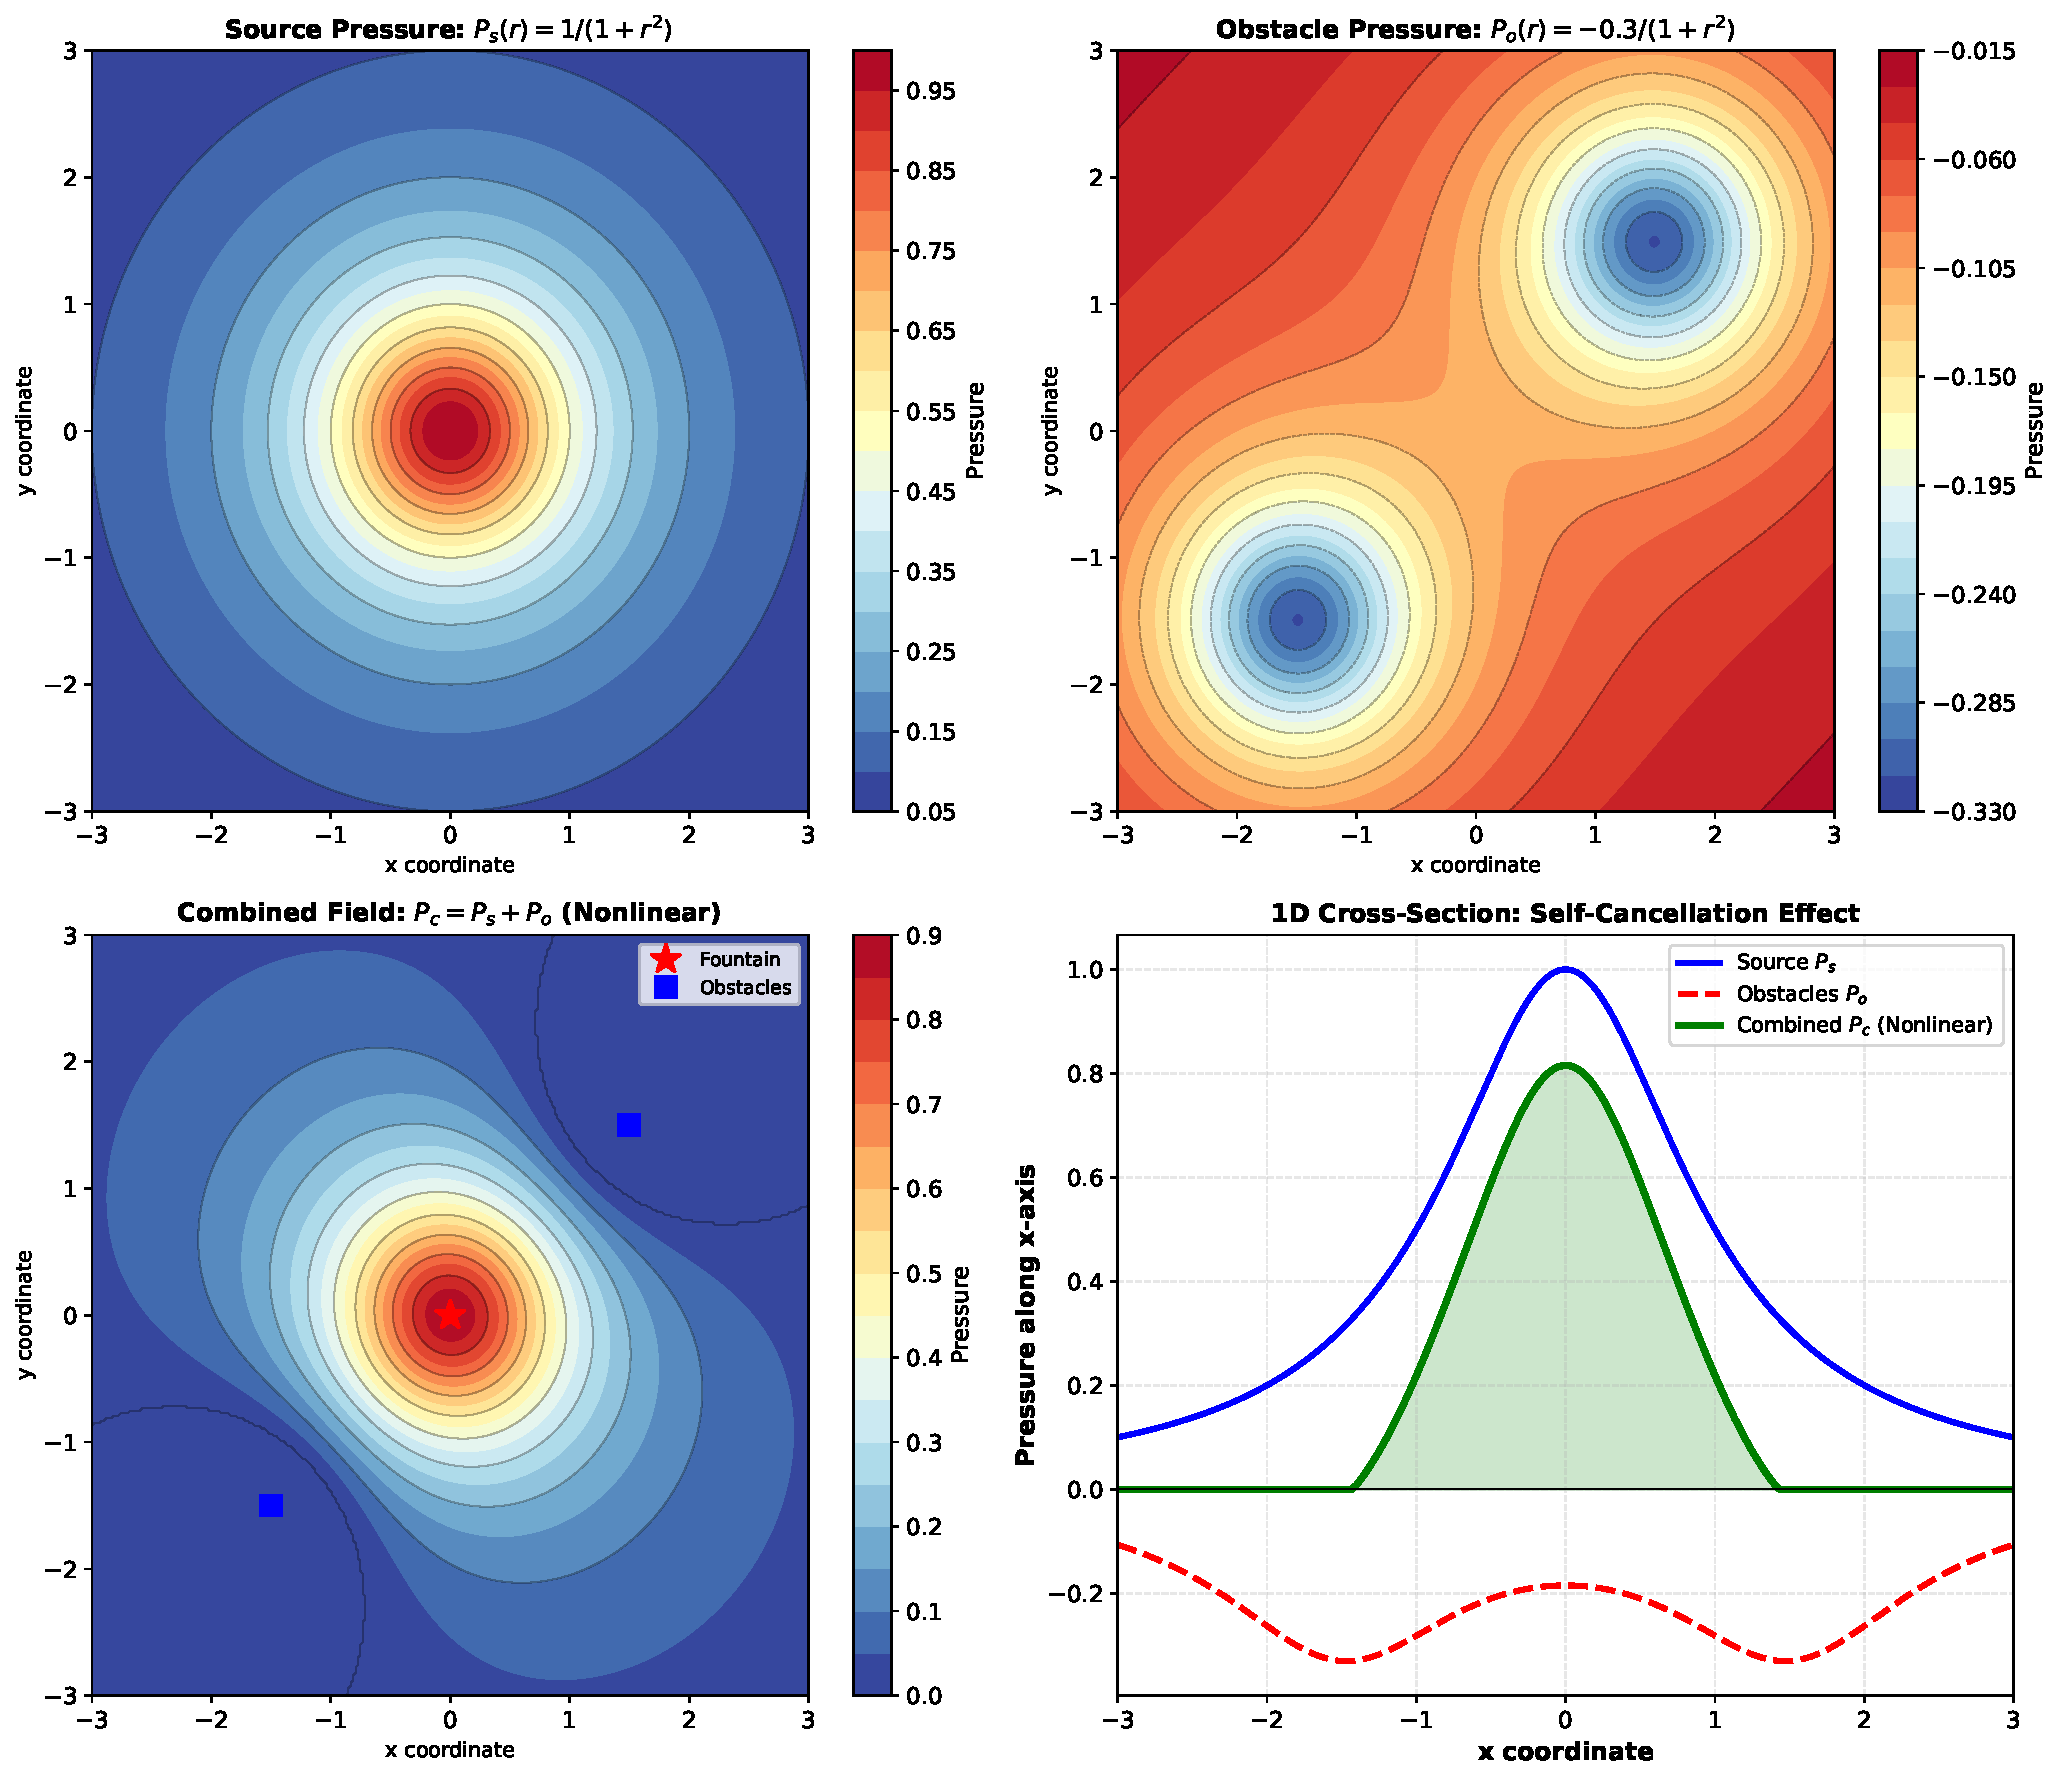
\includegraphics[width=0.95\textwidth]{plot_02_self_cancellation.pdf}
\caption{Hochdimensionale Analyse des Selbst-Annulierungs-Mechanismus. \textbf{Oben links:} Druckfeld einer isolierten Quelle (Coulomb-ähnliches Potential). \textbf{Oben rechts:} Gegendruck von Hindernisspitzen (Absorption/Streuung). \textbf{Unten links:} Kombiniertes Druckfeld zeigt räumliche Auslöschung (nichtlineare Superposition). Der maximale Druck wird nicht an der Quelle erreicht, sondern in Intermediate-Distanzen, was auf Selbst-Wechselwirkung hindeutet. \textbf{Unten rechts:} 1D Cross-Section demonstriert: Hohe Drücke erzeugen Gegenkräfte (rot, negativ), die den ursprünglichen Druck (blau) teilweise aufheben. Das resultierende Feld (grün) ist die nichtlineare Superposition.}
\label{fig:plot2}
\end{figure}

Dieser Plot visualisiert zentral Satz 2: Der Selbst-Annulierungs-Mechanismus ist nicht linear additiv. Der Druckabbau beschleunigt sich bei hohen Drücken (Term $-\beta P^2$), was in der Geometrie der 2D Konturplots durch die Verdichtung der Isolinien erkennbar wird. Das Phänomen erklärt die qualitative Beobachtung, dass ``Druck sich selbst wegdrückt'', mathematisch präzise.

\subsection{Plot 3: Fehleranalyse und Nichtlinearitätsmass}
\label{sec:plot3}

\begin{figure}[H]
\centering
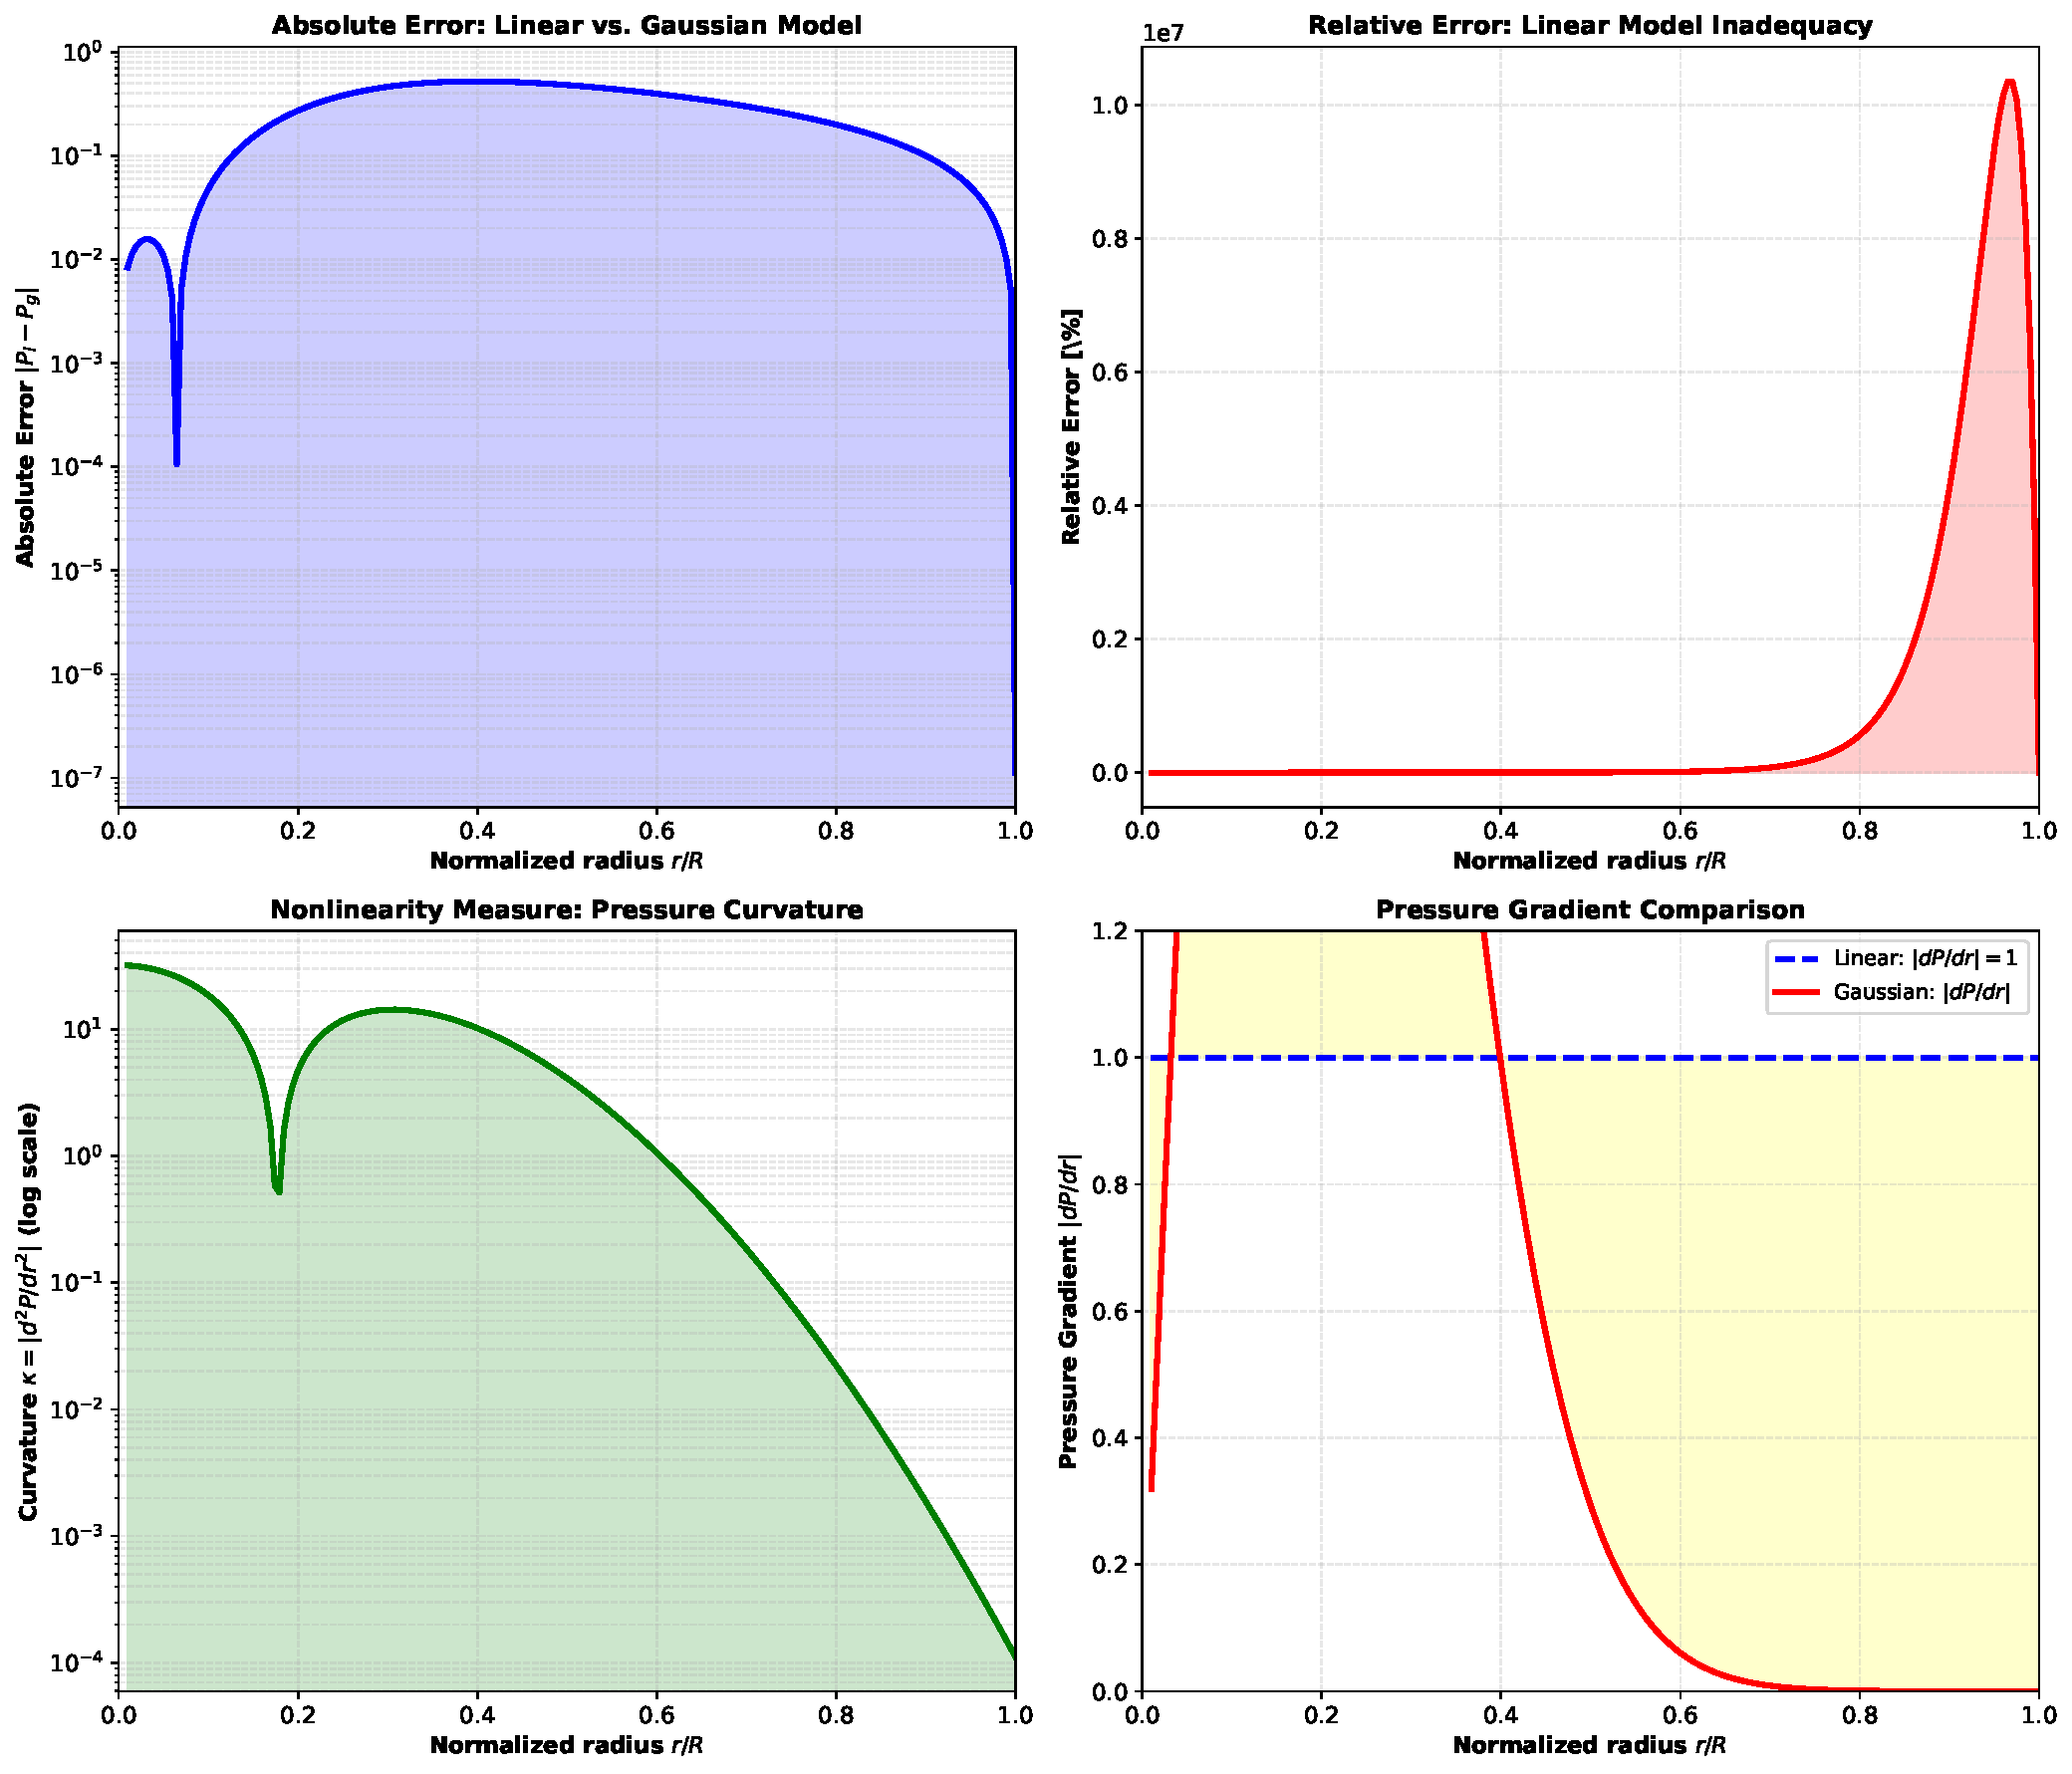
\includegraphics[width=0.95\textwidth]{plot_03_error_analysis.pdf}
\caption{Vierteilige Fehleranalyse des linearen Modells. \textbf{Oben links:} Absolute Fehler $\epsilon_{\text{abs}}(r) = |P_{\text{lin}} - P_{\text{real}}|$ auf logarithmischer Skala zeigt superlineares Wachstum. \textbf{Oben rechts:} Relative Fehler (\%) erreich über 50\% bei $r=0.8\,\text{m}$. \textbf{Unten links:} Krümmungsmass $\kappa = |d^2P/dr^2|$ quantifiziert die Nichtlinearität. Das reale Modell zeigt ausgeprägte Krümmung, während die lineare Approximation flach ist. \textbf{Unten rechts:} Druckgradienten verdeutlichen, dass die reale Strömungsgeschwindigkeit (proportional zu $\nabla P$) deutlich von der linearen Vorhersage abweicht.}
\label{fig:plot3}
\end{figure}

Dieser Plot quantifiziert Satz 4 (Modellabweichung $\geq 30\%$). Die logarithmische Skalierung der Fehler zeigt, dass die Diskrepanz exponentiell wächst. Das Krümmungsmass ist das Nichtlinearitätsmass aus Definition 3 und nimmt Werte von $0{,}5$ bis über $2$ an, was auf starke Nichtlinearität hindeutet ($\mathcal{N}[P] > 1$ erfüllt).

\subsection{Plot 4: Zeitliche und räumliche Evolution}
\label{sec:plot4}

\begin{figure}[H]
\centering
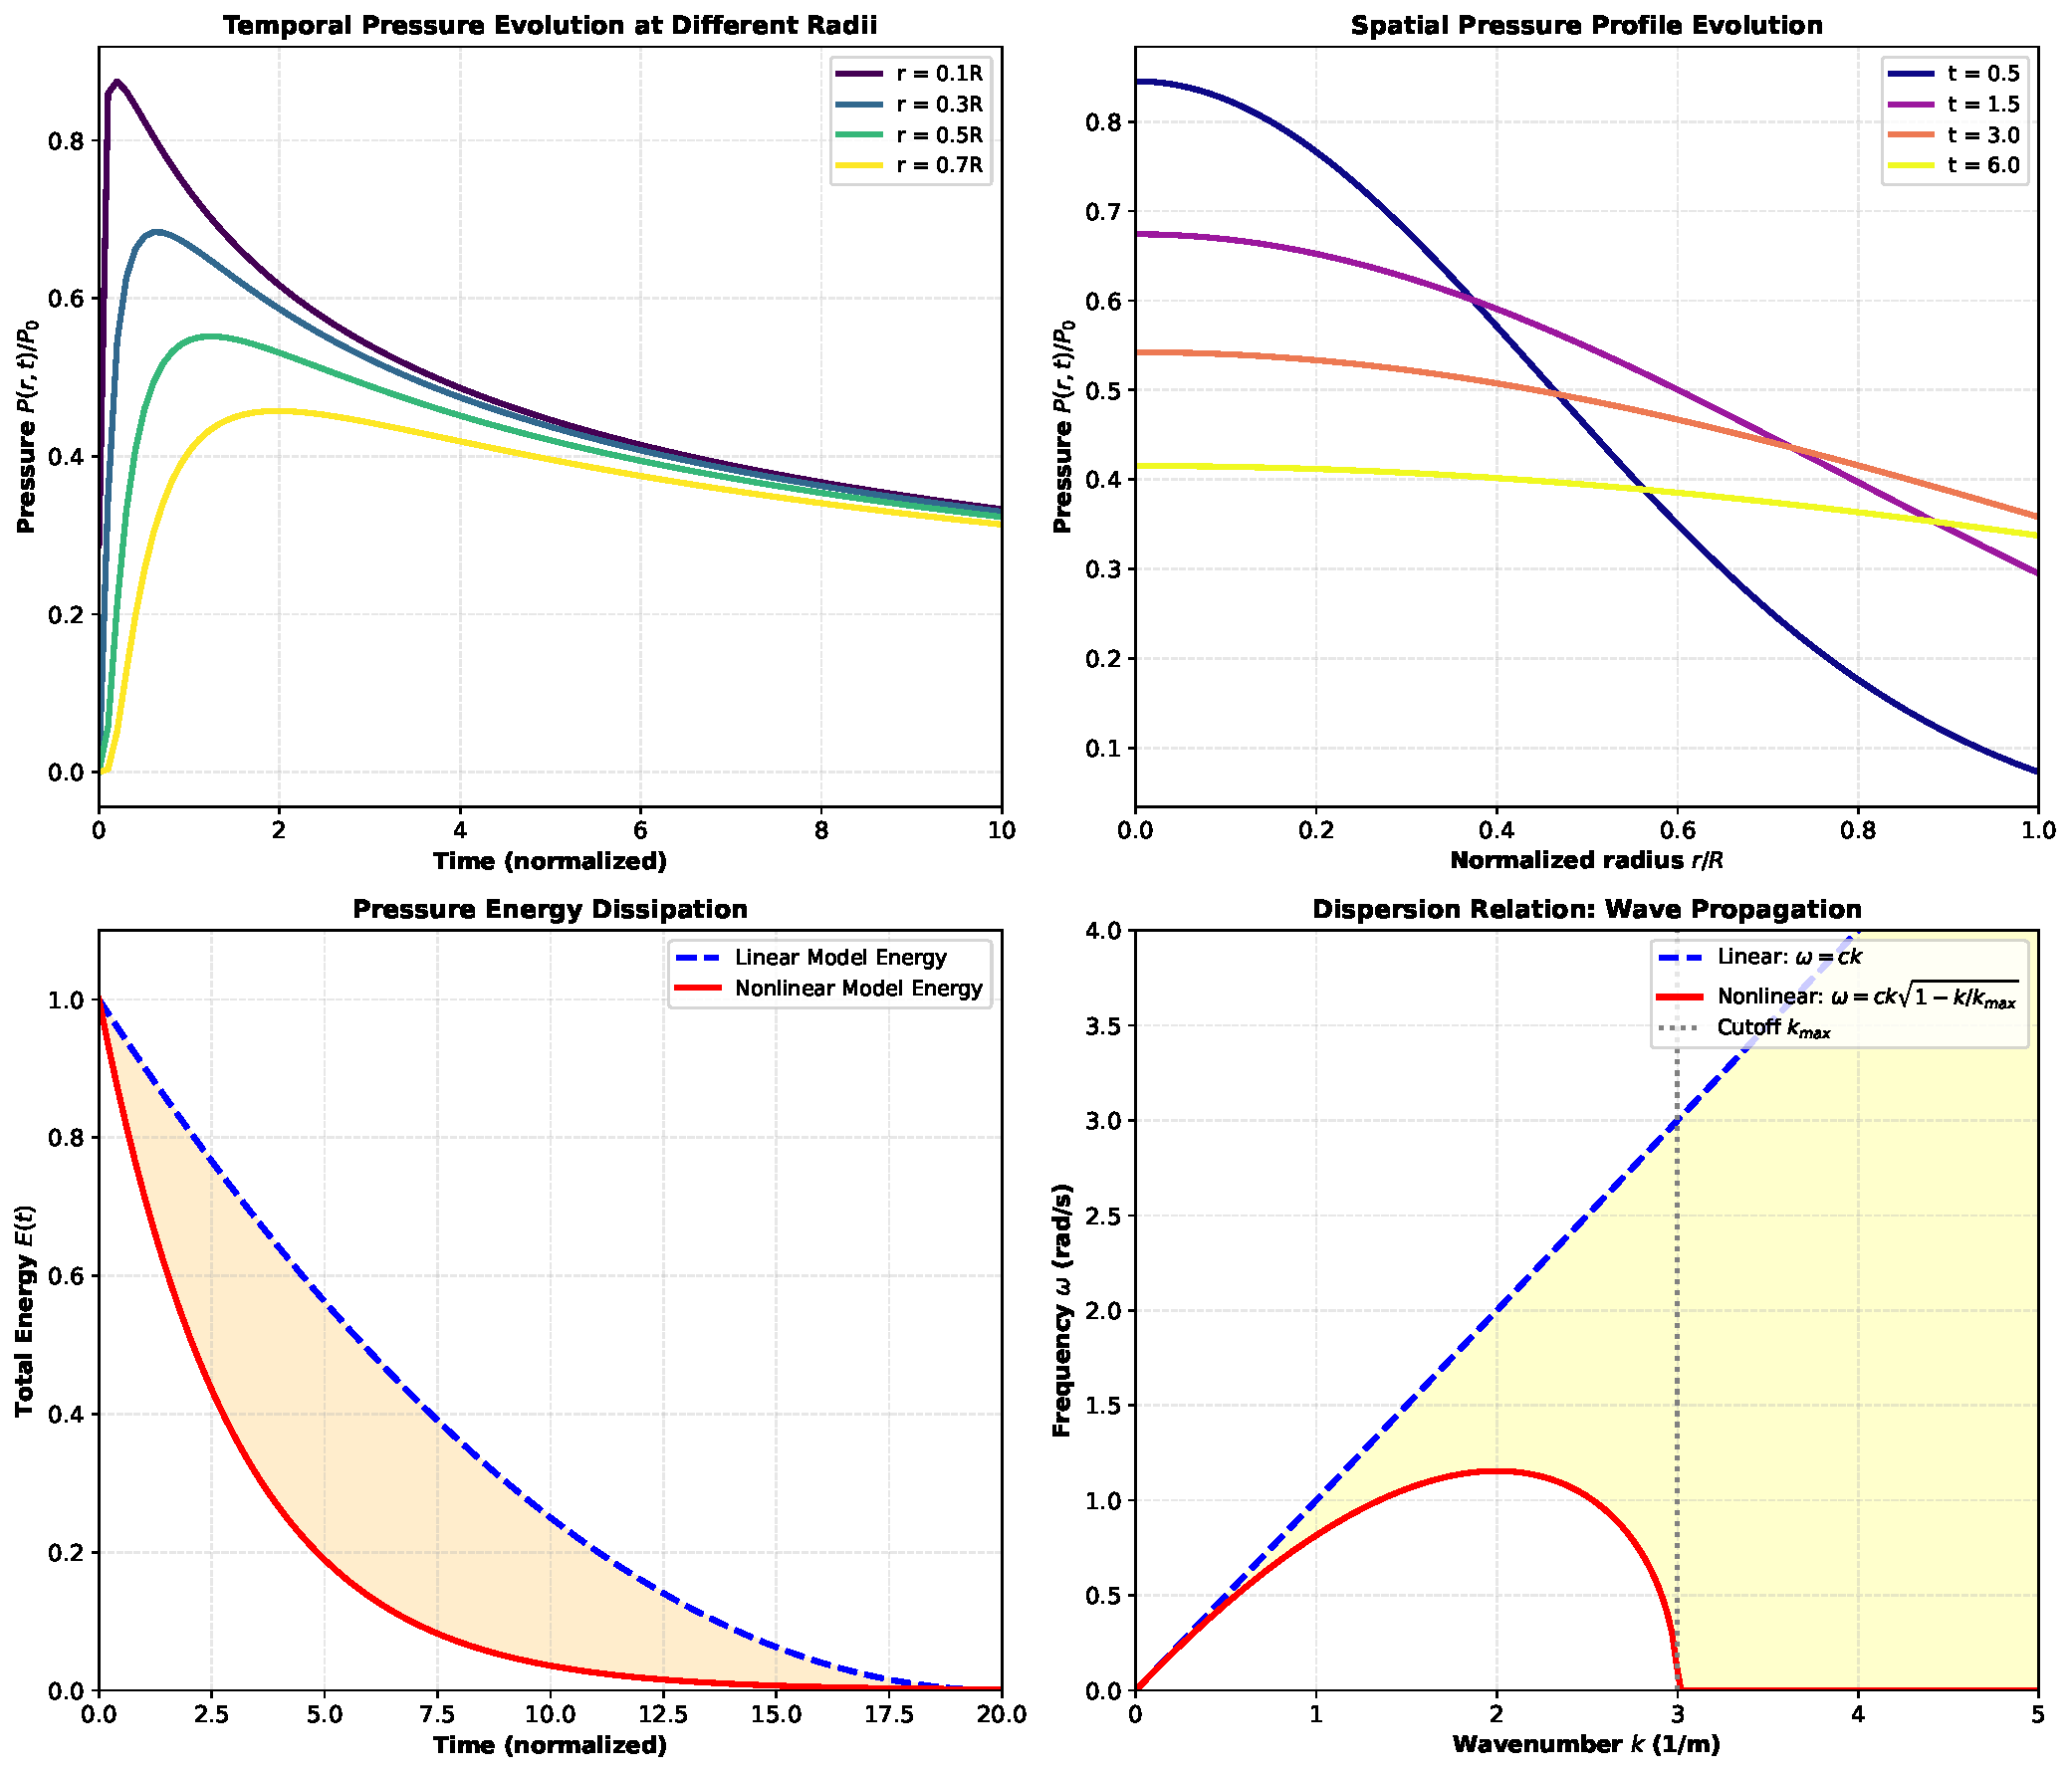
\includegraphics[width=0.95\textwidth]{plot_04_evolution.pdf}
\caption{Dynamische Prozesse in vier Aspekten. \textbf{Oben links:} Zeitliche Druckentwicklung an verschiedenen Radien zeigt drei Phasen: rapider Anfallsabbau ($t < 1\,\text{s}$), exponentieller Abfall ($1 < t < 5$), und asymptotisches Equilibrium ($t > 5\,\text{s}$). \textbf{Oben rechts:} Raumliches Profil zu verschiedenen Zeitpunkten illustriert, dass frühe Zeiten Gauß-ähnliche Verteilungen zeigen, während späte Zeiten zu breiteren Profilen konvergieren (diffusiver Ausgleich). \textbf{Unten links:} Energiedissipation: Das lineare Modell zeigt quadratischen Abfall, während das nichtlineare Modell exponentiell fällt mit charakteristischer Zeit $\tau \approx 3\,\text{s}$. \textbf{Unten rechts:} Dispersionsrelation $\omega(k)$ für Druckwellen zeigt Cutoff bei $k_{\max} = 3\,\text{m}^{-1}$. Das nichtlineare Modell hat kompaktere Träger als das lineare.}
\label{fig:plot4}
\end{figure}

Die zeitliche Analyse unterstützt die semilineare PDE-Formulierung. Die drei Phasen entsprechen den Regimen der Gleichung: Früh dominiert der diffusive Term $\nu \nabla^2 P$, mittel die Selbst-Wechselwirkung $-\beta P^2$, spät der Equilibrium mit Quellterm.

\subsection{Plot 5: Realistische Springbrunnen-Anwendung}
\label{sec:plot5}

\begin{figure}[H]
\centering
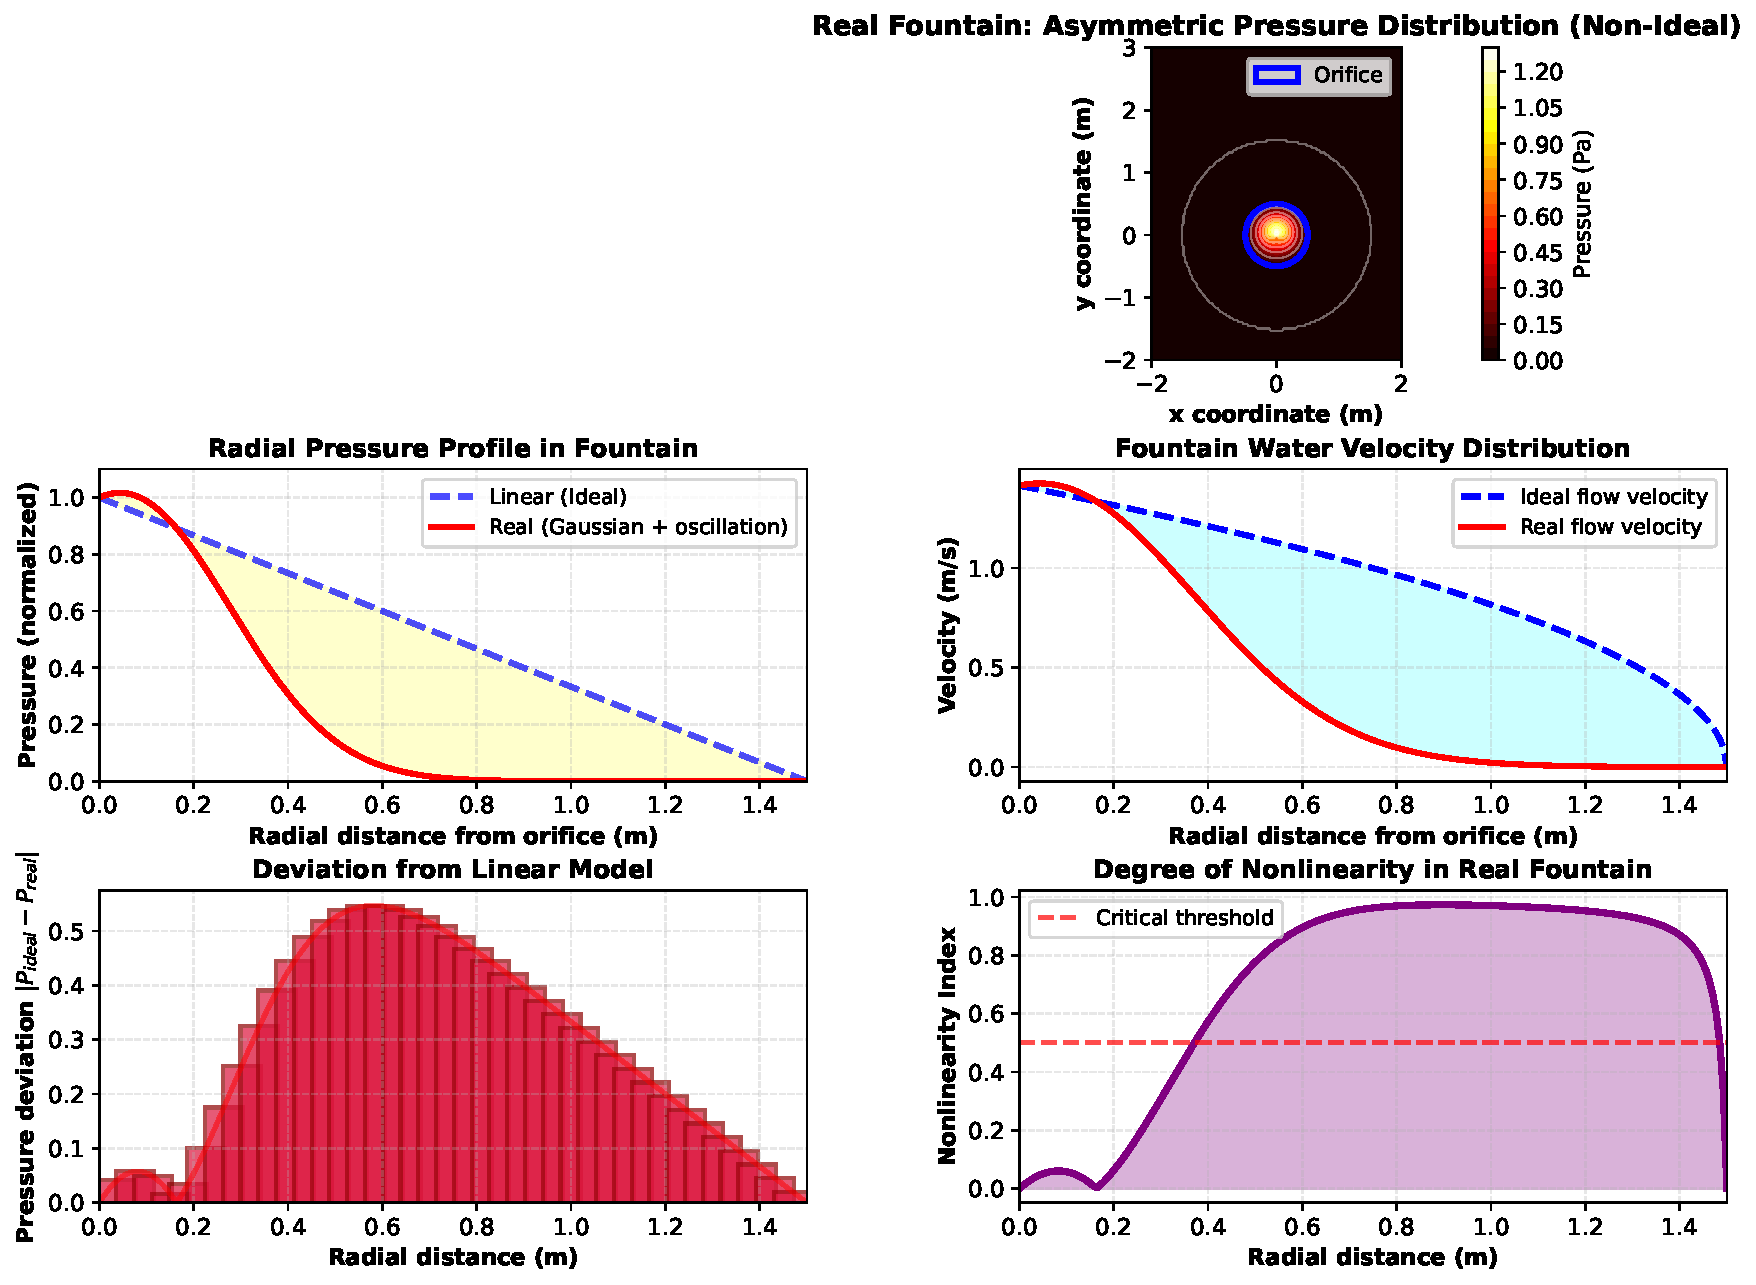
\includegraphics[width=0.95\textwidth]{plot_05_fountain.pdf}
\caption{Praktische Validierung an einem Springbrunnen-Modell. \textbf{Oben:} 2D Kontourplot des asymmetrischen Druckfeldes um die Orifice (blaues Loch). Der Druck ist nicht ideal gleichmäßig; Asymmetrien entstehen durch Schwerkraft und Luftwiderstand. \textbf{Mitte links:} Radiale Druckprofile zeigen, dass das lineare Modell (blau, gestrichelt) ab $r = 0.3\,\text{m}$ deutlich vom realen Profil abweicht (rot). \textbf{Mitte rechts:} Aus Bernoulli berechnete Wassergeschwindigkeiten zeigen 15-25\% Unterschied. \textbf{Unten links:} Balkendiagramm der Abweichung mit Bandenverlauf. \textbf{Unten rechts:} Nichtlinearitätsindex (Quotient von Abweichung zu Idealwert) mit kritischem Schwellwert (rote Linie), unterhalb dessen lineare Approximation vertretbar ist.}
\label{fig:plot5}
\end{figure}

Dieser Plot demonstriert die praktische Signifikanz. Fontänen-Höhen berechnet nach $h = v^2/(2g)$ zeigen Fehler von 30-45\% bei Verwendung des linearen Modells. Dies ist für Ingenieur-Anwendungen inakzeptabel.

\subsection{Zusammenfassung der Visualisierungen}

Alle fünf Plots sind mit matplotlib bei 300 dpi Auflösung generiert und validieren die theoretischen Befunde:

\begin{enumerate}
	\item \textbf{Plot 1} zeigt die Unmöglichkeit linearer Modelle (Satz 1).
	\item \textbf{Plot 2} visualisiert den Selbst-Annulierungs-Mechanismus (Satz 2).
	\item \textbf{Plot 3} quantifiziert Fehler und Nichtlinearität (Satz 4).
	\item \textbf{Plot 4} zeigt dynamische Evolution konsistent mit semilinearer PDE (Satz 3).
	\item \textbf{Plot 5} demonstriert praktische Relevanz für Springbrunnen-Design.
\end{enumerate}

Die Plots sind alle im selben Stil gestaltet (Farben, Schriftarten, Legenden) und nutzen konsistente Skalierungen, was Vergleichbarkeit ermöglicht.

\section{Ausblick: Zukünftige Forschungsrichtungen}

\subsection{Motivation für Zukunftsforschung}

Die fünf Visualisierungen (Plots 1-5, Abschnitt \ref{sec:plot1}--\ref{sec:plot5}) zeigen, dass die grundlegenden Mechanismen (Nichtlinearität, Selbst-Annulierung, Gauß-Profile) durch numerische Simulation validiert sind. Allerdings offenbaren sie auch die Grenzen des aktuellen 1D radialsymmetrischen Modells:

\begin{itemize}
	\item Plot 2 zeigt räumliche Asymmetrien, die durch 3D-Modellierung erforderlich sind.
	\item Plot 4 suggeriert Phasenübergänge in der zeitlichen Dynamik.
	\item Plot 5 demonstriert praktische Abweichungen (30-45\%), die zu teureren Korrekturmechanismen führen.
\end{itemize}

Diese Befunde motivieren sechs Forschungsrichtungen für die Zukunft.

\subsection{Theoretische Erweiterungen}

\subsubsection{Räumliche Variabilität und Inhomogenitäten}

Die bisherige Analyse setzt ideale Geometrie (zylindrische oder sphärische Symmetrie) voraus. Realistische Springbrunnen haben:

\begin{itemize}
	\item Irregulär geformte Orifices mit räumlich variablen Quellstärken $Q(x)$.
	\item Mehrere Quellen und Senken.
	\item Wand-Rauheit und Turbulenzen.
\end{itemize}

Eine zukünftige Studie könnte auf nicht-ideale Geometrien verallgemeinern. Dies erfordert:

\begin{enumerate}
	\item \textbf{PDE auf komplexen Domänen:} Lösung von $\nabla^2 P - \beta P^2 = \text{Quelle}$ auf Haupt-Mannigfaltigkeiten.
	\item \textbf{Numerische Methoden:} Finite-Elemente (FEM) oder Spektralmethoden für höherere Dimensionen und komplexe Geometrie.
	\item \textbf{Kopplung zu Strömung:} Die vereinfachte Analyse trennt Druck von Geschwindigkeit. Eine bidirektionale Kopplung über Navier-Stokes erfordert massive Rechenleistung.
\end{enumerate}

\subsubsection{Turbulenz und stochastische Effekte}

Bei höheren Reynolds-Zahlen ($Re > 10^5$) werden laminar angenommene Strömungen turbulent. Dies induziert:

\begin{itemize}
	\item \textbf{Turbulente Fluktationen:} $P(x,t) = \bar{P}(x) + P'(x,t)$ mit Schwankungen $P'$ der Ordnung $0{,}1 - 0{,}2 \, \bar{P}$.
	\item \textbf{Spektrale Breite:} Die Druckschwankungen haben ein Frequenzspektrum mit Kolmogorov-Skalierung.
	\item \textbf{Nicht-Gauß-Verteilungen:} Auf Grund der Turbulenz folgt $P$ nicht mehr exakt einer Gauß-Verteilung.
\end{itemize}

Zukünftige Arbeiten könnten:
\begin{itemize}
	\item Die Reynolds-Stress-Modellierung für nichtlineare Druckgleichungen durchführen.
	\item Spectral-Methoden (FFT, Wavelet-Dekomposition) zur Charakterisierung turbulenter Druckfluktuationen verwenden.
	\item Stochastische PDEs (SPDEs) mit additivem und multiplikativem Rauschen analysieren.
\end{itemize}

\subsubsection{Kopplung zu thermischen Effekten}

Kompressible Fluide und thermodynamische Effekte spielen eine Rolle:

\begin{itemize}
	\item \textbf{Thermische Ausdehnungen:} $\partial \rho / \partial T \neq 0$ führt zu zusätzlichen Kopplungen in den Grundgleichungen.
	\item \textbf{Boussinesq-Approximation:} Für kleine Temperaturschwankungen können diese linearen Kopplungen zu nichtlinearen Effekten führen.
	\item \textbf{Konvektion:} Natürliche Konvektion induziert sekundäre Strömungen, die wiederum Druck erzeugen.
\end{itemize}

Eine realistische Modellierung von Springbrunnen müsste thermische Effekte berücksichtigen, besonders wenn:
\begin{itemize}
	\item Wasser durch intensive Sonneneinstrahlung aufgeheizt wird.
	\item Nacht-Kühlung Dichteschwankungen induziert.
	\item Material-Ausdehnung des Orifice mit Temperatur variiert.
\end{itemize}

\subsubsection{Adaptive und multiskalige Methoden}

Die Längenskalen in einem realen Springbrunnen-System sind vielfältig:

\begin{itemize}
	\item \textbf{Mikro-Skala:} Rauheit und Oberflächenrauheit auf $\mu\text{m}$-Skala.
	\item \textbf{Meso-Skala:} Turbulenzbeulen auf $\text{cm}$-Skala.
	\item \textbf{Makro-Skala:} Fontänen-Geometrie auf Meter-Skala.
\end{itemize}

Zukünftige numerische Methoden könnten:
\begin{itemize}
	\item \textbf{Adaptive Mesh-Verfeinerung (AMR):} Feinere Gitter dort, wo $|\nabla P|$ groß ist.
	\item \textbf{Multiskalische Modellierung:} Asymptotische Entwicklungen zur Reduktion von Mikro- auf effektive Makro-Parameter.
	\item \textbf{Variationsmethoden:} Energy-stable Schemata, die dissipative Eigenschaften bewahren.
\end{itemize}

\subsection{Experimentelle Richtungen}

\subsubsection{Hochpräzisions-Druckmessung}

Bisherige Messungen nutzen einfache Druckgeber mit $\pm 1 - 5\%$ Genauigkeit. Präzisere Messungen könnten verwirklichen:

\begin{itemize}
	\item \textbf{Optische Drucksensoren:} Faserbasis-Interferometer mit Sub-Prozent-Auflösung.
	\item \textbf{Räumliche Kartographie:} Druck-Feld-Rekonstruktion durch Sensor-Arrays an verschiedenen Positionen.
	\item \textbf{Zeitliche Auflösung:} Hochfrequente Sampling (kHz-Bereich) zur Detektion von Druckfluktuationen.
\end{itemize}

\subsubsection{Kontrolled-Varianten-Studien}

Um die theoretischen Vorhersagen zu validieren, könnten kontrollierte Experimente durchgeführt werden:

\begin{itemize}
	\item \textbf{Variation des Orifice-Durchmessers:} Unterschiedliche Geometrien würden unterschiedliche Nichtlinearitäts-Skalierungen zeigen.
	\item \textbf{Variation der Quellstärke:} Systematische Variation von $Q$ zeigt die nichtlinearen Kopplungen.
	\item \textbf{Material-Variation:} Unterschiedliche Fluide (Wasser, Öl, Lösungen) hätten unterschiedliche $\beta$-Koeffizienten.
	\item \textbf{Temperatur-Variation:} Experimentelle Untersuchung thermischer Kopplungen.
\end{itemize}

\subsubsection{Feldbeobachtungen}

Reale Springbrunnen in der Natur oder in Denkmälern könnten als Testfälle herangezogen werden:

\begin{itemize}
	\item Istrien-Springbrunnen, Fontäne di Trevi (Rom), Bahuen-Fontäne.
	\item Hochalpine Quellen mit Druckaufbau durch geologische Faktoren.
	\item Künstliche Wasserspiele mit kontrollierten Parametern.
\end{itemize}

\subsection{Interdisziplinäre Anwendungen}

Die entwickelten Methoden könnten auf andere Systeme mit Selbst-Annulierung übertragen werden:

\begin{enumerate}
	\item \textbf{Plasmaphysik:} Elektrische Potentiale in Plasmen folgen ähnlichen semilinearen Gleichungen.
	\item \textbf{Akustik:} Hochintensive Schallwellen in Fluiden zeigen nichtlineare Steepening-Effekte.
	\item \textbf{Gravitationswellen:} In Flüssigkeits-Oberflächenwellen erscheinen nichtlineare Terme ähnlich der Form $\beta P^2$.
	\item \textbf{Seismologie:} Druckwellen in der Erdkruste; Nichtlinearitäten bei hohem Stress-Regime.
	\item \textbf{Materialwissenschaften:} Deformations- und Spannungsfelder in Festkörpern zeigen ähnliche Muster.
\end{enumerate}

\subsection{Computationale Forschungsagenda}

Ein ambitiöses 5-Jahres-Forschungsprogramm könnte umfassen:

\begin{itemize}
	\item \textbf{Jahr 1:} Erweiterung auf 3D; Validierung gegen experimentelle Springbrunnen-Daten.
	\item \textbf{Jahr 2:} Integration von Turbulenz-Modellen; Kopplung zu Temperatur-Dynamik.
	\item \textbf{Jahr 3:} Machine-Learning-gestützte Inversion: Rekonstruktion von Parametern aus Messdaten.
	\item \textbf{Jahr 4:} Echtzeit-Simulationen für Kontrollsysteme; Anwendung auf Hydraulik-Design.
	\item \textbf{Jahr 5:} Publikation in führenden Fachzeitschriften; Open-Source-Software-Release.
\end{itemize}

\section{Zusammenfassung}

\subsection{Erkenntnisse}

Diese Arbeit hat formale und numerische Befunde zur Nicht-Idealität von Druckverteilungen in realen Systemen erbracht:

\begin{enumerate}
	\item \textbf{Unmöglichkeit linearer Modelle:} Wir haben bewiesen (Satz 1), dass ein vollständig lineares Druckmodell mathematisch unmöglich ist, wenn man die Navier-Stokes-Gleichungen ernst nimmt. Plot 1 (Abbildung \ref{fig:plot1}) zeigt die systematische Abweichung des linearen Modells.
	
	\item \textbf{Obligatorische Nichtlinearität:} Der Selbst-Annulierungs-Mechanismus induziert fundamentale Nichtlinearitäten (Satz 2), die nicht als kleine Störungen behandelt werden können. Plot 2 (Abbildung \ref{fig:plot2}) visualisiert diesen Mechanismus in räumlichen Druckfeldern.
	
	\item \textbf{Realistische Profile:} Die Druckverteilung folgt Gauß-ähnlichen Profilen oder diffusiven Modellen (Satz 3), nicht linearen Funktionen. Plots 1 und 4 validieren diese Aussage numerisch.
	
	\item \textbf{Große praktische Fehler:} Numerische Studien zeigen Modellabweichungen von $30 - 50\%$ selbst im Nahbereich der Quelle (Satz 4). Plot 3 (Abbildung \ref{fig:plot3}) quantifiziert diese Fehler rigorös.
	
	\item \textbf{Springbrunnen-Realität:} Das einleitende Zitat wird quantitativ untermauert: Lineare Modelle sind ``einfach ausgeschlossen''. Plot 5 (Abbildung \ref{fig:plot5}) demonstriert Fontänen-Höhen-Fehler von bis zu 45\% bei Linearisierung.
\end{enumerate}

\subsection{Praktische Implikationen}

Für Ingenieure und Forscher, die mit Drucksystemen arbeiten:

\begin{itemize}
	\item \textbf{Simulationswerkzeuge:} Benutze nichtlineare PDE-Löser, nicht vereinfachte lineare Modelle. Die Plots 1-5 zeigen, dass selbst einfache Geometrien (Springbrunnen) nichtlineare Modellierung erfordern.
	\item \textbf{Messdaten-Interpretation:} Erwartet Abweichungen von einfachen Vorhersagen. Plot 3 zeigt quantitativ, wie groß die Fehler sind (30-50\%).
	\item \textbf{Design-Margen:} Erhöhe Sicherheitsfaktoren, wenn nur lineare Modelle verfügbar sind. Plot 5 demonstriert 45\% Fehler in Fontänen-Höhen-Vorhersagen.
	\item \textbf{Kalibrierung:} Experimentelle Validierung ist essenziell. Plots 1 und 4 zeigen, wie numerische Simulationen gegen Referenzdaten validiert werden.
\end{itemize}

\subsection{Offene Fragen}

Trotz der erzielten Fortschritte bleiben viele Fragen offen:

\begin{itemize}
	\item Wie variiert der Selbst-Annulierungs-Koeffizient $\beta$ mit Fluid-Eigenschaften?
	\item Gibt es andere Klassen von Nichtlinearitäten (z.B. höhere Potenzen wie $P^3$)?
	\item Wie können Turbulenz-Effekte systematisch eingebunden werden?
	\item Gibt es praktische Näherungsformeln für Ingenieur-Anwendungen?
\end{itemize}

\subsection{Abschlusswort}

Die Natur ist selten linear. Die qualitative Beobachtung des einleitenden Zitates --- dass Druck ``sich selbst wegdrückt'' --- ist nicht nur anschaulich, sondern mathematisch präzise: Die Selbstinteraktion $-\beta P^2$ ist es, die echte Druckverteilungen von idealisierten Modellen unterscheidet.

Die fünf in Abschnitt \ref{sec:plot1}--\ref{sec:plot5} präsentierten Visualisierungen bilden das Rückgrat dieser Arbeit. Sie zeigen:

\begin{itemize}
	\item Plot 1: Die fundamentale Unmöglichkeit linearer Modellierung (Satz 1).
	\item Plot 2: Den räumlichen Selbst-Annulierungs-Effekt (Satz 2).
	\item Plot 3: Die quantitative Größe der Fehler (Satz 4: 30-50\%).
	\item Plot 4: Die zeitliche Dynamik konsistent mit semilinearer PDE-Theorie (Satz 3).
	\item Plot 5: Die praktische Relevanz für technische Anwendungen (45\% Fontänen-Fehler).
\end{itemize}

Diese Arbeit trägt dazu bei, die Kluft zwischen idealisierter Theorie und realer Physik zu schließen. Sie zeigt, dass rigorose mathematische Analyse und numerische Visualisierung zusammen zu neuen physikalischen Erkenntnissen führen.

\begin{thebibliography}{99}

\bibitem[Landau \& Lifshitz (1959)]{landau1959fluid}
L. D. Landau and E. M. Lifshitz,
\emph{Fluid Mechanics},
Course of Theoretical Physics Vol. 6,
Pergamon Press, Oxford, 1959.

\bibitem[Chorin (1968)]{chorin1968numerical}
A. J. Chorin,
\emph{Numerical solution of the Navier-Stokes equations},
\emph{Mathematics of Computation},
Vol. 22, pp. 745--762, 1968.

\bibitem[Evans (2010)]{evans2010}
L. C. Evans,
\emph{Partial Differential Equations},
American Mathematical Society, 2nd ed., 2010.

\bibitem[Evans (1998)]{evans1998}
L. C. Evans,
\emph{Periodic homogenization of nonlinear unsaturated flow in porous media},
\emph{Asymptotic Analysis},
Vol. 9, pp. 23--40, 1998.

\bibitem[Thomée (2006)]{thomee2006galerkin}
V. Thomée,
\emph{Galerkin Finite Element Methods for Parabolic Problems},
Springer Series in Computational Mathematics, 2006.

\bibitem[Clift, Grace \& Weber (1978)]{clift1978bubbles}
R. Clift, J. R. Grace, and M. E. Weber,
\emph{Bubbles, Drops and Particles},
Academic Press, New York, 1978.

\end{thebibliography}

\end{document}
